\documentclass[conference]{IEEEtran}
\IEEEoverridecommandlockouts

% Packages from the IEEE conference template.
\usepackage{amsmath,amssymb,amsfonts}
\usepackage{algorithmic}
\usepackage{graphicx}
\usepackage{textcomp}
\usepackage{xcolor}
\usepackage{array}
\usepackage{url}
\usepackage{tikz}
\usepackage{pgfplots}
\usepackage{float}
\pgfplotsset{compat=1.18}
\usepackage[
  colorlinks=true,
  linkcolor=black,
  citecolor=black,
  urlcolor=blue,
  filecolor=black,
  pdfborder={0 0 0}
]{hyperref}

% Bibliography setup.
% Compile with Biber.
\usepackage[style=ieee,backend=biber,sorting=none]{biblatex}
\addbibresource{citations.bib}

\def\BibTeX{{\rm B\kern-.05em{\sc i\kern-.025em b}\kern-.08em
    T\kern-.1667em\lower.7ex\hbox{E}\kern-.125emX}}

\begin{document}

\title{A Comparative Study of Fine-Tuned Lightweight LLMs for Automated Code Smell Detection}

\author{
\IEEEauthorblockN{Fatema Kotb, Ahmed Emad, Rofayda Bassem, Mahinour Elsarky, and Mostafa Abdelbarr}
\IEEEauthorblockA{
\textit{Computer Engineering Program, Faculty of Engineering, Cairo University}\\
Cairo, Egypt\\
\begin{tabular}{c}
fatema.kotb02@eng-st.cu.edu.eg, ahmedemad8@gmail.com, rofaydabassem@gmail.com\\
mahinouralaa2002@gmail.com, mostafa.abdelbrr@gmail.com
\end{tabular}
}
}

\maketitle

\begin{abstract}
This paper presents a comparative analysis of small, locally deployable language models for automated code smell detection. Using the MLCQ dataset, a benchmark of ~13,400 manually labeled Java code reviews, we formulate the task as binary classification, predicting whether a code smell is present or absent in each code sample. Four lightweight models with distinct architectures are compared: Qwen3-0.6B, Qwen3-1.7B, Llama-3.2-1B-Instruct, and Gemma-3-1B-it, all fine-tuned using Low-Rank Adaptation (LoRA) under a consistent experimental setup. Performance is evaluated primarily using the present-class F1-score, as it directly reflects the ability to detect actual code smells in an imbalanced dataset. Results show that Qwen3-1.7B achieves the highest present-class F1-score of 0.6021, followed closely by Gemma-3-1B-it at 0.56. These findings suggest that small, fine-tuned models can serve as practical alternatives to large-scale language models for software quality tasks, particularly in settings where local deployment and limited computing are real constraints.
\end{abstract}

\begin{IEEEkeywords}
automated code smell detection, MLCQ, language models, LoRA, fine-tuning, F1-score
\end{IEEEkeywords}

\section{Introduction}
\label{sec:introduction}

\subsection{Background}
\label{subsec:background}
Software projects are growing over time and have multiple developers working on a large codebase. Having inefficient or poor design negatively impacts maintainability and readability which could cost valuable resources like time and money. These are known as code smells, which has been a major ongoing research topic in software engineering. They can be deceptive as code can function correctly because they don’t appear as bugs however they indicate design problems that can make the system hard to interpret, modify, scale, test and evaluate. The early detection of code smells is very important to point out for any needed refactoring and prevent the accumulation of bad code design. 
Examples of code smells include God Class, where a single class takes on too many responsibilities; Long Method, where a method grows too long and hard to read; Feature Envy, where a method relies more on another class's data than its own; and Data Class, which just holds data but doesn't do anything meaningful with it. These four smells span both class-level and method-level concerns and represent some of the most frequently studied categories in the literature. Detecting code smells matters because they may harm:
\begin{itemize}
    \item Maintainability: smelly code is harder to modify without introducing new issues.
\end{itemize}
\begin{itemize}
    \item Readability: developers spend more time understanding poorly structured code.
\end{itemize}
\begin{itemize}
    \item Testability: tightly coupled or overly complex code is difficult to test in isolation.
\end{itemize}

\subsection{Motivation}
\label{subsec:motivation}
Early stages required manual code smell detection which was considered very costly and time-consuming due to the need for experienced developers to review code carefully which doesn’t scale as projects grow in size and complexity. This motivated research into finding automated code smell detection solutions. It started with heuristic-based rules and manual metrics and although it was straightforward, this was very difficult to generalize across different kinds of projects, languages and smell types as well as the need of significant domain expertise.
With the rise of Artificial Intelligence (AI), Machine learning (ML) and Deep Learning (DL) techniques, code smell detection problems were treated as a classification problem that can learn complex patterns directly from code. More recently, NLP-based models and large language models (LLMs) offered stronger contextual understanding and improved detection performance further.
Despite these advances, they had a huge limitation which is their high computational cost and deployment complexity. In many real-world environments, running or even accessing LLMs is not feasible, especially where data privacy, limited hardware, or local deployment are required. In recent years, new generations of small light LLMs have become more popular where they are designed to run on standard hardware without requiring intensive resources and costs, yet their effectiveness on code quality tasks such as smell detection remain underexplored.

\subsection{Project Aim}
\label{subsec:project-aim}
This paper addresses the gap identified above by investigating whether small, locally deployable LLMs can achieve good performance on code-smell detection after fine-tuning. The main contribution is a comparative analysis showing evidence on how model size and architectural design affect classification performance across different code smell types, and whether small LLMs can be a good alternative to large-scale LLMs or not. This paper focuses on comparing four light LLMs with distinct architectures including Qwen3-0.6B, Qwen3-1.7B, Llama-3.2-1B-Instruct, and Gemma-3-1B-it.
All models are fine-tuned using LoRA on the MLCQ dataset, a benchmark of approximately ~13,400 manually labeled real-world Java code samples across four smell categories mentioned above. The task is formulated as binary classification, where the model predicts whether a code smell is present or absent for a given code sample and target smell type. The evaluation uses a consistent experimental setup across all models, with present-class F1-score as the primary comparison metric, since the main goal is detecting actual code smells and accuracy alone can be misleading given the class imbalance in the dataset.
\section{Dataset and Task Definition}
\label{sec:dataset-task}

\subsection{MLCQ Dataset}
\label{subsec:mlcq-dataset}
The dataset used in this study is \textbf{MLCQ}, an industry-relevant code smell dataset introduced by Madeyski and Lewowski \cite{madeyski2020mlcq}. The data were collected through a structured review process in which software developers assessed code samples extracted from actively developed Java open-source projects hosted on GitHub. Sample selection and review were supported by an acquisition tool developed by the authors, which presented either class-level or method-level code fragments to reviewers and recorded their assessments in a database. The data include four code smell types: Blob, Data Class, Feature Envy, and Long Method. The total number of samples is 4,770 collected from 523 projects and reviewed 14,739 times by 26 reviewers. Each record links a code sample with a smell type and its assigned label. The schema includes, among other fields, a sample identifier, reviewer identifier, smell type, severity label, review timestamp, sample type (class or method), code element name, and a link to the original source location. In this work, only the smell presence information is used, while the original severity annotations are converted into binary labels.

\subsection{Smells Included}
\label{subsec:smells-included}
In this paper, we are focusing on the four code smell types from the MLCQ dataset: Blob, Data Class, Feature Envy, and Long Method.

Blob and Data Class are class-level code smells, whereas Feature Envy and Long Method are method-level code smells. A Blob is a large class that accumulates too many responsibilities, while a Data Class mainly stores data and provides little meaningful behavior \cite{Jerzyk2023}. Feature Envy describes a method that appears to rely more on the data or functionality of another class than on those of its own class, whereas a Long Method is a method that becomes excessively large and therefore harder to understand, test, and maintain \cite{Jerzyk2023}.

\subsection{Task Definition}
\label{subsec:task-definition}
The task considered in this study is binary code smell detection. As described later in Subsection~\ref{subsec:dataset}, each input is formed by combining a code sample from the dataset with a specific smell type. The model then determines whether that smell is present in the given sample. Because this study does not address the severity annotations available in the original dataset, the prediction space is limited to two labels: \textit{present} and \textit{absent}.
\section{Related Work}
\label{sec:related-work}

\subsection{Earlier Heuristic-Based Approaches}

Code smell detection focused mainly on heuristic-based techniques and software metrics. These methods identified smells using predefined rules, threshold values, and metric combinations extracted from source code. Rule-based detection became widely used because it was relatively simple to apply and automate. However, the quality of detection often depended on how thresholds were selected and how the rules were designed, which could vary between projects and developers \cite{mesbah2025nlp,zhang2024peftsmells}.

Heuristic-based methods also had difficulty handling the semantic side of source code. In practice, some methods with high complexity values were still easy for developers to read and maintain, while other problematic code fragments were missed because they did not cross predefined metric thresholds. Because of this, rule-based detectors did not always match developers’ judgment when identifying code smells.

\subsection{Machine Learning and Deep Learning Approaches}

To overcome some of the limitations of rule-based detection, later studies introduced machine learning techniques for code smell detection. In these approaches, the problem was treated as a classification task in which models learned to distinguish between smelly and non-smelly code using labeled examples. Many early machine learning methods relied on handcrafted software metrics and used traditional classifiers such as Random Forests, Support Vector Machines, and decision trees.

With the growth of deep learning, researchers began using models that learn patterns directly from source code instead of relying only on manually extracted metrics. Several neural network architectures, such as CNNs, LSTMs, BiLSTMs, and GNNs, were later applied to better capture both the structure and meaning of code. Compared with earlier metric-based approaches, these models reduced the amount of manual feature engineering required and showed improved capability in handling more complex code patterns \cite{mesbah2025nlp}.

Research using the MLCQ dataset showed that pretrained code representations could improve code smell detection performance compared with traditional heuristic-based methods. Several studies reported that machine learning approaches achieved stronger performance than traditional metric-based detectors in multiple evaluation settings, supporting the idea that learned representations are more suitable for identifying complex smells.

\subsection{NLP and Pretrained Language Models}

Mesbah et al. compared several architectures, including LSTM, BiLSTM, and attention-based models, on smells such as Feature Envy, Data Class, Blob, and Long Method. Their experiments on the MLCQ dataset showed that BiLSTM models combined with attention mechanisms achieved stronger performance than simpler recurrent architectures in several smell categories.

The study also experimented with pretrained transformer models, including CodeBERT, and compared them with other NLP-based approaches. The experiments showed that pretrained models performed well in some detection tasks without depending much on manually designed features. However, the results differed between smell types, since certain smells were easier for the models to identify than others. Other research explored embeddings generated from models such as code2vec, code2seq, CuBERT, CodeT5, and CodeBERT for representing source code in smell detection tasks \cite{mesbah2025nlp}.

\subsection{Large Language Models and Parameter-Efficient Fine-Tuning}

Large Language Models were later explored in several software engineering tasks, especially code generation and code summarization. Although these models showed strong general coding capabilities, earlier experiments on code smell detection reported weaker performance when the models were applied directly without task-specific training. This led researchers to study different fine-tuning approaches for improving smell detection results.

One recent study investigated parameter-efficient fine-tuning (PEFT) methods for code smell detection. Zhang et al. introduced a source-code-centric benchmark containing Complex Conditional, Complex Method, Feature Envy, and Data Class smells, and evaluated PEFT techniques such as prompt tuning, prefix tuning, and LoRA. Their experiments showed that PEFT methods could match or sometimes outperform full fine-tuning while requiring fewer trainable parameters and lower GPU memory usage \cite{zhang2024peftsmells}.

At the same time, newer open-source language model families such as Qwen3 provided smaller coding-oriented models that are more practical for limited computational environments. The Qwen3 series includes models ranging from 0.6B to 235B parameters and reported improvements on coding and reasoning benchmarks \cite{qwen32025report}.  


\section{Methodology}
\label{sec:methodology}

\subsection{Dataset}
\label{subsec:dataset}

We first loaded the original MLCQ dataset~\cite{madeyski2020mlcq}, in which each row represents a review. Each review contains a review ID, reviewer ID, sample ID, smell type, and the severity assigned by the reviewer. The severity takes one of the following values: critical, major, minor, or none. The dataset also includes metadata fields that can be combined to access the corresponding sample through GitHub.

\subsubsection{Label Generation}

Since our problem is binary classification per smell type, we are only concerned with whether or not the sample has the target smell, not the severity of the smell. For this reason, we mapped the severity values into binary labels. The severity level none was mapped to absent, while all other severity levels were mapped to present. The review-level severity distribution before binary conversion is shown in Table~\ref{tab:severity-distribution}.

\begin{table}[t]
\caption{Review-level severity distribution by code smell type.}
\label{tab:severity-distribution}
\centering
\begin{tabular}{lrrrr}
\hline
Smell Type & Critical & Major & Minor & None \\
\hline
Blob & 127 & 312 & 535 & 3,045 \\
Data Class & 146 & 401 & 510 & 2,964 \\
Feature Envy & 24 & 142 & 288 & 2,883 \\
Long Method & 78 & 274 & 454 & 2,556 \\
\hline
\end{tabular}
\end{table}

\subsubsection{Sample Retrieval}

We then attempted to fetch all 4,770 samples used across the 14,739 reviews. Of these samples, 4,364 were retrieved successfully, while 406 returned HTTP 404 errors, meaning that the corresponding repository locations could no longer be accessed. This left us with 13,444 usable reviews, while 1,295 reviews were discarded.

\subsubsection{Class Imbalance}

For each smell type, we compared the number of reviews labelled as present with those labelled as absent. As shown in Fig.~\ref{fig:class-imbalance}, the dataset is highly imbalanced, with the absent label appearing much more often than the present label. We accounted for this imbalance during training, as explained in Section~\ref{subsubsec:class-weighting}.

\begin{figure}[t]
\centering
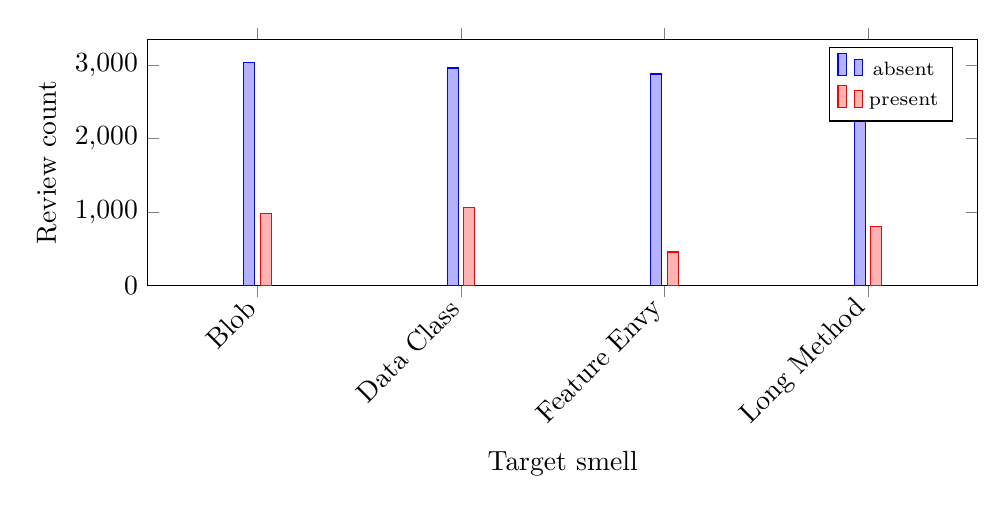
\begin{tikzpicture}
\begin{axis}[
    ybar,
    width=\columnwidth,
    height=4.7cm,
    bar width=4pt,
    ylabel={Review count},
    xlabel={Target smell},
    symbolic x coords={Blob,Data Class,Feature Envy,Long Method},
    xtick=data,
    x tick label style={rotate=45,anchor=east},
    ymin=0,
    legend style={at={(0.97,0.97)},anchor=north east,font=\scriptsize},
    enlarge x limits=0.18
]
\addplot coordinates {(Blob,3045) (Data Class,2964) (Feature Envy,2883) (Long Method,2556)};
\addplot coordinates {(Blob,974) (Data Class,1057) (Feature Envy,454) (Long Method,806)};
\legend{absent,present}
\end{axis}
\end{tikzpicture}
\caption{Review-level binary label distribution by code smell type.}
\label{fig:class-imbalance}
\end{figure}

\subsection{Data Preprocessing}
\label{subsec:data-preprocessing}

\subsubsection{Prompt Construction}

After retrieving the samples, we created a prompt for each review to use as the model input. The prompt asks the model to determine whether the sample contains the target smell type. It includes the smell type being evaluated, the source code associated with the sample, and the expected output format.

\subsubsection{Reviewer Disagreement}

After preprocessing, we had 8,711 unique sample-smell pairs, 1,007 of which had reviewer disagreement. This means that, for some sample-smell pairs, different reviewers assigned severities that were mapped to different binary labels.

To stay consistent with how the MLCQ dataset is normally used, and to make our results comparable with earlier research, we did not remove the samples with reviewer disagreement. Therefore, the dataset remained review-based instead of being reduced to one final label for each sample-smell pair.

The number of unique sample-smell pairs is greater than the number of samples because each sample could be reviewed with respect to up to two smell types.

\subsubsection{Train/Validation/Test Split and Leakage Prevention}

To avoid data leakage, we split the data by sample rather than by review. When splitting the data using a 70/15/15 ratio, we made sure that all reviews of the same sample were placed in the same split. This means that the same sample cannot appear in more than one of the training, validation, and test sets.

We ended up with 9,383, 2,034, and 2,027 reviews in the training, validation, and test splits, respectively. These add up to the full set of 13,444 usable reviews. We also recorded the label distribution and smell type distribution in each split (Table~\ref{tab:split-distribution}) to check that the split did not introduce major bias.

\begin{table}[t]
\caption{Train, validation, and test label distribution.}
\label{tab:split-distribution}
\centering
\begin{tabular}{lrrr}
\hline
Split & Reviews & Absent & Present \\
\hline
Train & 9,383 & 7,332 & 2,051 \\
Validation & 2,034 & 1,580 & 454 \\
Test & 2,027 & 1,565 & 462 \\
\hline
\end{tabular}
\end{table}

The cleaned dataset was then saved and used for training and evaluating the models.

\subsection{Model Training}
\label{subsec:model-training}

We used the same configurations and pipeline for training all models, with very few exceptions that are explicitly documented in this work. The training and optimization settings used across the experiments are summarized in Table~\ref{tab:training-config}. The binary classification setup and LoRA configuration are summarized in Table~\ref{tab:lora-config}.

The training of all models was done on a Tesla T4 GPU available on free Kaggle accounts.

\subsubsection{Model Selection}

The models trained in this work are:

\begin{itemize}
\item Qwen/Qwen3-0.6B
\item Qwen/Qwen3-1.7B
\item meta-llama/Llama-3.2-1B-Instruct
\item google/gemma-3-1b-it
\item deepseek-ai/DeepSeek-R1-Distill-Qwen-1.5B
\end{itemize}

All selected models are lightweight LLMs with fewer than 2B parameters.

\subsubsection{Class Weighting}
\label{subsubsec:class-weighting}

We first loaded the cleaned dataset that was saved after preprocessing. Then, we used only the training split to calculate the class weights.

The class weights were calculated using the formula:

\[
\text{class\_weight} = \frac{\text{total training examples}}{\text{number of classes} \times \text{class count}}
\]

where \texttt{number\_of\_classes} is 2, since the labels are absent and present, and \texttt{class\_count} is the number of training examples belonging to the class we are calculating the weight for.

These weights were then used in weighted cross entropy during training. We did this to reduce the effect of the class imbalance discussed earlier. Without using class weights, the model could mostly predict the majority class, which is absent, and still get a relatively high accuracy. The weights came out to around 0.64 for the absent class and 2.29 for the present class, which reflects the imbalance between the two labels.

\subsubsection{Tokenisation and Input Preparation}

Before training, the prompts were converted into token sequences using the tokenizer associated with each model. This was necessary because the selected models do not all use the same vocabulary or tokenisation scheme, so each prompt had to be represented in the format expected by the model being trained.

For consistency across all experiments, the maximum input length was set to 512 tokens. Prompts that exceeded this limit were truncated before being passed to the model.

Shorter inputs were padded during batching so that examples with different lengths could be processed together. Padding was applied at the batch level, while truncation was applied during tokenisation.

\subsubsection{Model Architecture and Parameter-Efficient Fine-Tuning}

Each selected model was adapted for binary sequence classification. Given an input prompt, the model outputs scores for two possible labels: absent and present.

Instead of fully fine-tuning all model parameters, we used LoRA as a parameter-efficient fine-tuning method. With this approach, most of the original model parameters remain frozen, and only a small number of additional trainable parameters are updated during training. This reduces the memory and computational cost of fine-tuning.

In our setup, LoRA was applied to the query and value projection modules in the attention layers. A classification head with two outputs was used to produce scores for the absent and present labels. For Qwen/Qwen3-0.6B, this resulted in 1,148,928 trainable parameters out of 597,200,896 total parameters, meaning that only 0.1924\% of the parameters were updated during training.

This setup allowed us to fine-tune all selected lightweight LLMs using the same general training pipeline while keeping the experiments feasible within the available computational resources.

\subsection{Evaluation Metrics}
\label{subsec:evaluation-metrics}

We calculated accuracy, precision, recall, and F1 score on the training, validation, and test sets, with the results reported per smell type. Since the dataset is imbalanced, we paid particular attention to the results for the present class. Insights from these results are discussed in Section~\ref{sec:results}.

The meaning and calculation of each metric are also provided in Table~\ref{tab:evaluation-metrics}.

\begin{table}[t]
\caption{Evaluation metrics and their calculations.}
\label{tab:evaluation-metrics}
\centering
\begin{tabular}{>{\raggedright\arraybackslash}p{0.24\linewidth}>{\raggedright\arraybackslash}p{0.63\linewidth}}
\hline
Metric & Calculation \\
\hline
Accuracy & $(TP + TN) / (TP + TN + FP + FN)$ \\
Precision & $TP / (TP + FP)$ \\
Recall & $TP / (TP + FN)$ \\
F1-score & $2 \times (\text{Precision} \times \text{Recall}) / (\text{Precision} + \text{Recall})$ \\
\hline
\end{tabular}
\end{table}

\section{Results and Discussion}
\label{sec:results}

\subsection{Overall Test Performance}
\label{subsec:overall-test-performance}
\begin{table}[h!]
\centering
\caption{Model performance on the test set using present-class precision, recall, and F1-score}
\label{tab:model-performance}
\begin{tabular}{|l|c|c|c|c|}
\hline
\textbf{Model} & \textbf{Accuracy} & \textbf{Precision} & \textbf{Recall} & \textbf{F1-score} \\
\hline
Qwen3-0.6B & 0.7790 & 0.5139 & 0.5584 & 0.5353 \\
\hline
Qwen3-1.7B & 0.7528 & 0.4755 & 0.8203 & 0.6021 \\
\hline
Llama-3.2-1B-Instruct & 0.7538 & 0.4632 & 0.5043 & 0.4829 \\
\hline
Gemma-3-1B-it & 0.7449 & 0.4614 & 0.7121 & 0.5600 \\
\hline
\end{tabular}
\end{table}
Code smell detection focuses on recall as an important metric because we want a model that can correctly identify actual code smells. However, precision is also important, since we do not want too many false alarms. Therefore, we rank the models primarily by their F1-score.
Accuracy cannot be relied on as the main metric because of the class imbalance, with many more ``absent'' instances than ``present'' ones.
As shown in Table~\ref{tab:model-performance}, Qwen3-1.7B achieves the highest overall F1-score, followed by Gemma-3-1B-it, Qwen3-0.6B, and Llama-3.2-1B-Instruct.
The differences between the models are moderate, but the best-performing model may vary when performance is examined by code smell type, as shown in Table~\ref{tab:smell-type-f1}.

\subsection{Performance by Code Smell Type}
\label{subsec:performance-by-smell}
To better understand model behavior across different smell categories, we compare the Present F1-score for each code smell type, as shown in Table~\ref{tab:smell-type-f1}.
\textit{Qwen3-1.7B} achieves the best F1-score for Blob, Data Class, and Feature Envy, while \textit{Gemma-3-1B-it} performs best for Long Method. Overall, \textit{Qwen3-1.7B} is the strongest model in most cases, but the best-performing model changes slightly depending on the code smell type.

\begin{table}[htbp]
\centering
\caption{Performance by code smell type using present-class F1-score}
\label{tab:smell-type-f1}
\small
\resizebox{\columnwidth}{!}{%
\begin{tabular}{lcccc}
\hline
\textbf{Model} & \textbf{Blob} & \textbf{Data Class} & \textbf{Feature Envy} & \textbf{Long Method} \\
\hline
Qwen3-0.6B & 0.4586 & 0.5260 & 0.2581 & 0.7953 \\
Qwen3-1.7B & 0.6187 & 0.5371 & 0.3429 & 0.8333 \\
Llama-3.2-1B-Instruct & 0.3922 & 0.4227 & 0.3143 & 0.7431 \\
Gemma-3-1B-it & 0.5296 & 0.4970 & 0.2941 & 0.8369 \\
\hline
\end{tabular}%
}
\end{table}

\subsection{Easiest and Hardest Code Smells}
\label{subsec:easiest-hardest-smells}

To identify which code smells are easier or harder to detect overall, we calculate the average Present F1-score for each smell type across all four models, as shown in Table~\ref{tab:average-smell-f1}.

\begin{table}[h]
\centering
\caption{Average Present F1-score across models for each code smell type}
\label{tab:average-smell-f1}
\begin{tabular}{lc}
\hline
Smell Type & Average F1 Across Models \\
\hline
Blob & 0.499768 \\
Data Class & 0.495689 \\
Feature Envy & 0.302332 \\
Long Method & 0.802143 \\
\hline
\end{tabular}
\end{table}

Long Method is the easiest code smell to detect overall, achieving the highest average F1-score of 0.802143. In contrast, Feature Envy was the hardest code smell to detect overall in our results  with the lowest average F1-score of 0.302332. This may be because identifying Feature Envy often requires broader structural and semantic context, such as understanding how a method interacts with other classes and whether its behavior is misplaced. The MLCQ data set suggests that highly severe cases are relatively rare, with only a small number of instances rated as critical by developers with industrial experience \cite{madeyski2020mlcq}.

\section{Conclusion}
\label{sec:conclusion}
In this paper, comparative analysis has been done on four small LLMs, Qwen3-0.6B, Qwen3-1.7B, Llama-3.2-1B-Instruct and Gemma-3-1B-it. These LLMs were fine-tuned with LoRA for binary code smell detection on the MLCQ dataset. The main goal is to find evidence that small light models can perform well in detecting code smells without the need for high resources and computation.
The results of this study show that Qwen3-1.7B achieved the best overall present-class F1-score of 0.6021, ranking first on three out of four smell types (Blob, Data Class, and Feature Envy). Gemma-3-1B-it came in second overall and did the best on detecting Long Method code smells. These results show that small language models can detect code smells well enough to be useful even when they are trained on a single free-tier GPU.
The performance of these language models varied a lot depending on the type of code smell. Long Method was the easiest to detect, with a F1-score of 0.80 across all models. This is probably because Long Method code smells are easier to spot since they are usually very long. On the other hand, Feature Envy was the hardest to detect with an average F1-score of only 0.30 since detecting feature envy requires understanding how parts of the code work together which can be more challenging.
One of the limitations of this study is that it only compared four language models that were fine-tuned in the same way. Different fine-tuning methods, prompt formats, or other settings could have given different results. Moreover, the MLCQ dataset focused on Java code from open-source projects, which means the results may not generalize to other languages or codebases.
Future work could explore different LoRA configurations and hyperparameter settings, since these can affect model performance. It would also be worth evaluating the models on datasets that include other programming languages.

\section*{Acknowledgment}
Insert acknowledgments here, or delete this section.

\appendices
\section{Training and LoRA Configuration}
\label{app:training-config}

This appendix summarizes the training and LoRA settings used in the experiments. The same general configuration was used across the lightweight LLMs, with the model checkpoint changed for each experiment.

\begin{table}[H]
\centering
\caption{Training and Optimization Configuration}
\label{tab:training-config}
\begin{tabular}{ll}
\hline
Setting & Value \\
\hline
Seed & 42 \\
Maximum input length & 512 tokens \\
Number of epochs & 3 \\
Learning rate & $2 \times 10^{-4}$ \\
Training batch size & 16 \\
Evaluation batch size & 32 \\
Gradient accumulation steps & 2 \\
Weight decay & 0.01 \\
Warmup ratio & 0.03 \\
Learning-rate scheduler & Linear \\
Maximum gradient norm & 1.0 \\
\hline
\end{tabular}
\end{table}

\begin{table}[H]
\centering
\caption{Task and LoRA Configuration}
\label{tab:lora-config}
\begin{tabular}{ll}
\hline
Setting & Value \\
\hline
Task setup & Binary sequence classification \\
Output labels & absent, present \\
Positive class & present \\
PEFT method & LoRA \\
LoRA rank & 8 \\
LoRA alpha & 16 \\
LoRA dropout & 0.05 \\
LoRA target modules & \texttt{q\_proj}, \texttt{v\_proj} \\
\hline
\end{tabular}
\end{table}


\printbibliography

\end{document}
